% last updated in April 2002 by Antje Endemann
% Based on CVPR 07 and LNCS, with modifications by DAF, AZ and elle, 2008 and AA, 2010, and CC, 2011; TT, 2014; AAS, 2016

\documentclass[runningheads]{llncs}
\usepackage{graphicx}
\usepackage{amsmath,amssymb} % define this before the line numbering.
\usepackage{ruler}
\usepackage{booktabs}
\usepackage[usenames, dvipsnames]{color}
\usepackage[width=122mm,left=12mm,paperwidth=146mm,height=193mm,top=12mm,paperheight=217mm]{geometry}
\usepackage{hyperref}

\usepackage{xspace}

\newcommand{\sz}[1]{\textcolor{blue}{\emph{//sz: #1//}}}
\newcommand{\cs}[1]{\textcolor{PineGreen}{\emph{//cs: #1//}}}
\newcommand{\la}[1]{\textcolor{cyan}{\emph{//la: #1//}}}

\newcommand{\vgenome}{VisualGenome\xspace}
\newcommand{\referit}{ReferIt\xspace}
\newcommand{\refcoco}{RefCOCO\xspace}
\newcommand{\refcocop}{RefCOCO+\xspace}
\newcommand{\flickr}{Flickr30k Entities\xspace}

\newcommand{\refexp}[1]{\textsl{#1}}
\newcommand{\word}[1]{\textsl{#1}}
\newcommand{\cat}[1]{\textsc{#1}}

\newcommand{\green}[1]{\textcolor{PineGreen}{#1}}
\newcommand{\red}[1]{\textcolor{red}{#1}}
\newcommand{\blue}[1]{\textcolor{blue}{#1}}
\newcommand{\yellow}[1]{\textcolor{yellow}{#1}}

\usepackage{pifont}
\newcommand{\cmark}{\ding{51}}%
\newcommand{\xmark}{\ding{55}}

\begin{document}
% \renewcommand\thelinenumber{\color[rgb]{0.2,0.5,0.8}\normalfont\sffamily\scriptsize\arabic{linenumber}\color[rgb]{0,0,0}}
% \renewcommand\makeLineNumber {\hss\thelinenumber\ \hspace{6mm} \rlap{\hskip\textwidth\ \hspace{6.5mm}\thelinenumber}}
% \linenumbers
\pagestyle{headings}
\mainmatter
\def\ECCV18SubNumber{***}  % Insert your submission number here

\title{Object naming is context-dependent - A case study on testing linguistic hypotheses on real-world image corpora} % Replace with your title

\titlerunning{ECCV-18 submission ID \ECCV18SubNumber}

\authorrunning{ECCV-18 submission ID \ECCV18SubNumber}

\author{Anonymous ECCV submission}
\institute{Paper ID \ECCV18SubNumber}


\maketitle

\begin{abstract}
Massive data collections for applications in language \& vision are nowadays available. In principle, these could constitute valuable resources also for research in computational linguistics (CL), besides task-specific modeling. However, in practice, very few studies have tested linguistic hypotheses using these large-scale datasets. In this paper, we illustrate the challenges of using this type of corpora for CL research, by focusing on a case study, namely the context-dependence of object naming in real-world images. Our analysis of existing resources in language \& vision reveals that none of the available datasets consistently satisfies all of the requirements for a linguistically motivated study of this phenomenon. We conclude with a proposal for a more consistent annotation of language \& vision data which can aid the study of object naming.
%The abstract should summarize the contents of the paper. LNCS guidelinesindicate it should be at least 70 and at most 150 words. It should be set in 9-point font size and should be inset 1.0~cm from the right and left margins.
\keywords{Object naming, object categorization, concepts, entry-level categories}
\end{abstract}

%@Carina TODO:
%\begin{itemize}
%	\item requirements: \\ 
%	add most specific name; (possible ways to obtain information: taxonomy, object detectors) \\
%	add unconstraint object co-occurrences / unbiased as far as possible; \\
%	rename R1? (lexical alternatives? candidate names?)
%	\item title?
%\end{itemize}

\section{Introduction}

Understanding and modeling the way humans converse about their environment using natural language has been a long-standing goal of research in various fields related to artificial intelligence and (computational) linguistics.
With recent  developments in computer vision and a range of massive data collections in particular, there has been a veritable explosion of interest in language \& vision (L\&V) tasks, ranging from image captioning \cite{fangetal:2015,devlin:imcaqui,Bernardietal:automatic}, referring expression resolution and generation \cite{Kazemzadeh2014,mao15,Yu2016}, to multi-modal summarization or visual dialogue \cite{das2017visual,vries2017guesswhat}.
In principle, the underlying data collections here should not only spur computational, application-oriented research aimed at implementing systems for very specific tasks---they should also constitute extremely valuable resources for research aimed at deriving linguistic generalizations about various phenomena related to language grounding, reference and situated interaction which, for a long time, have been investigated mostly in very controlled and small-domain experimental settings, cf. \cite{anderson1991hcrc,fernangen:sigd07,krahmer:2012,takenobu2012rex,zarriess2016pentoref} for some examples of traditional data collections related to reference and grounding.  
In turn, these linguistic generalizations could inform computational modeling, architecture design and future data collections.
However, so far, studies that have tested linguistic hypotheses on large-scale L\&V resources have been relatively rare. 


In this paper, we take a look at object naming, a core phenomenon that occurs in virtually every L\&V task and is, at the same time, subject of ongoing research in language grounding and pragmatics. 
Our starting point is a particular linguistic hypothesis related to object naming---namely that the choice of a name for an object is dependent on other objects in its visual context---which has been tested recently in a classical experimental setting \cite{graf2016animal}. 
We discuss how this hypothesis could be tested based on recent data sets that pair images and object descriptions, referring expressions or captions (all containing object names) and define a set of requirements for obtaining a theoretically informed model for object naming.
In sum, this discussion will show that specific requirements are met by particular resources, but none of the available corpora consistently 
satisfy 
all of the requirements.
We believe that this is a perfect showcase illustrating the challenges for linguistically motivated research in L\&V, and we derive a proposal for obtaining more consistently designed and annotated data collections for object naming.


\section{Naming Objects (in Context)}
\label{sec:object_naming}

The act of naming an object amounts to that of picking out a nominal to be employed to refer to it (e.g., ``the \refexp{dog}'', ``the white \refexp{dog} to the left'').
Since an object is simultaneously a member of multiple categories (e.g., a young \refexp{beagle} is at once a \cat{dog}, a \cat{beagle}, an \cat{animal}, a \cat{puppy} etc.), all the various names that lexicalize these constitute a valid alternative, meaning that the same object can be named with more or less \textbf{specific names} \cite{brown1958shall,murphy2004big}. 
Seminal work on concepts by Rosch suggests that object names typically exhibit a preferred level of specificity called the \textbf{entry-level}. This typically corresponds to an intermediate level of specificity, i.e., \textbf{basic level} (e.g, \refexp{bird}, \refexp{car}) \cite{rosch1976basic}, as opposed to more generic (i.e., \textbf{super-level}; e.g., \refexp{animal}, \refexp{vehicle}) or specific categories (i.e., \textbf{sub-level}; e.g., \refexp{sparrow}, \refexp{convertible}). However, less prototypical members of basic-level categories tend to be instead identified with sub-level categories (e.g., a \cat{penguin} is typically called a \refexp{penguin} and not a \refexp{bird}) \cite{jolicoeur1984pictures}. 
%This out-of-context preference towards a certain taxonomic level is often referred to as \textbf{lexical availability}. 
While the traditional notion of entry-level categories suggests that objects tend to be named by a \refexp{single} preferred concept, research on pragmatics has found that speakers are flexible in  
%with respect to the chose level of specificity. 
their choice of the level of specificity. 
Scenarios where multiple objects (of the same category) are present induce a pressure for generating names which uniquely identify the target \cite{olson1970language}, such that sub-level names can be systematically elicited in these cases %\cite{rohde2012communicating} \cite{graf2016animal}. 
\cite{rohde2012communicating}\cite{graf2016animal}.
For example, in presence of more than one dog, the name \textsl{dog} is ambiguous and a sub-level category (e.g., \textsl{rottweiler}, \textsl{beagle}) is more informative and potentially preferred by speakers, though additional factors such as cost or saliency also come into play \cite{graf2016animal}\cite{clark1983common}.
%Note that reasoning about the informativeness of a name require categorization of all the potential referents in that context (e.g., to know that \textit{dog} is ambiguous require having recognized that there are multiple dogs in the scene). 
%Other contextual factors affecting lexical choice include the \textbf{perceptual salience} of the object, such as its size or location \cite{clark1983common}.

So far, research in L\&V, has mostly worked around the fact that objects can be categorized and named at different levels of specificity.
 State-of-the-art object recognizers are typically trained on a flat set of categories taken from ImageNet, cf.\ \cite{googlenet}, though see work by Deng et al. on trading off object recognition accuracy and level of specificity \cite{deng2012hedging}.
\cite{Ordonez:2016} present one of the few explicit studies on naming in computer vision and operationalize the task as translating between leaf nodes in the ImageNet hierarchy and entry-level
 concepts, adopting the traditional view that there is a single preferred name for a given object that can be determined independently of the visual context.
 %Thus, establishing whether object naming is context dependent in realistic, large-scale data sets would not only be of interest to theoretical work on concepts and pragmatics, it would also be of great importance for the design of models in computer vision, object recognition and vision \& language.

\section{Requirements}
\label{sec:requirements}

\begin{figure}[t]
	\begin{center}
		\begin{minipage}{.35\textwidth}
			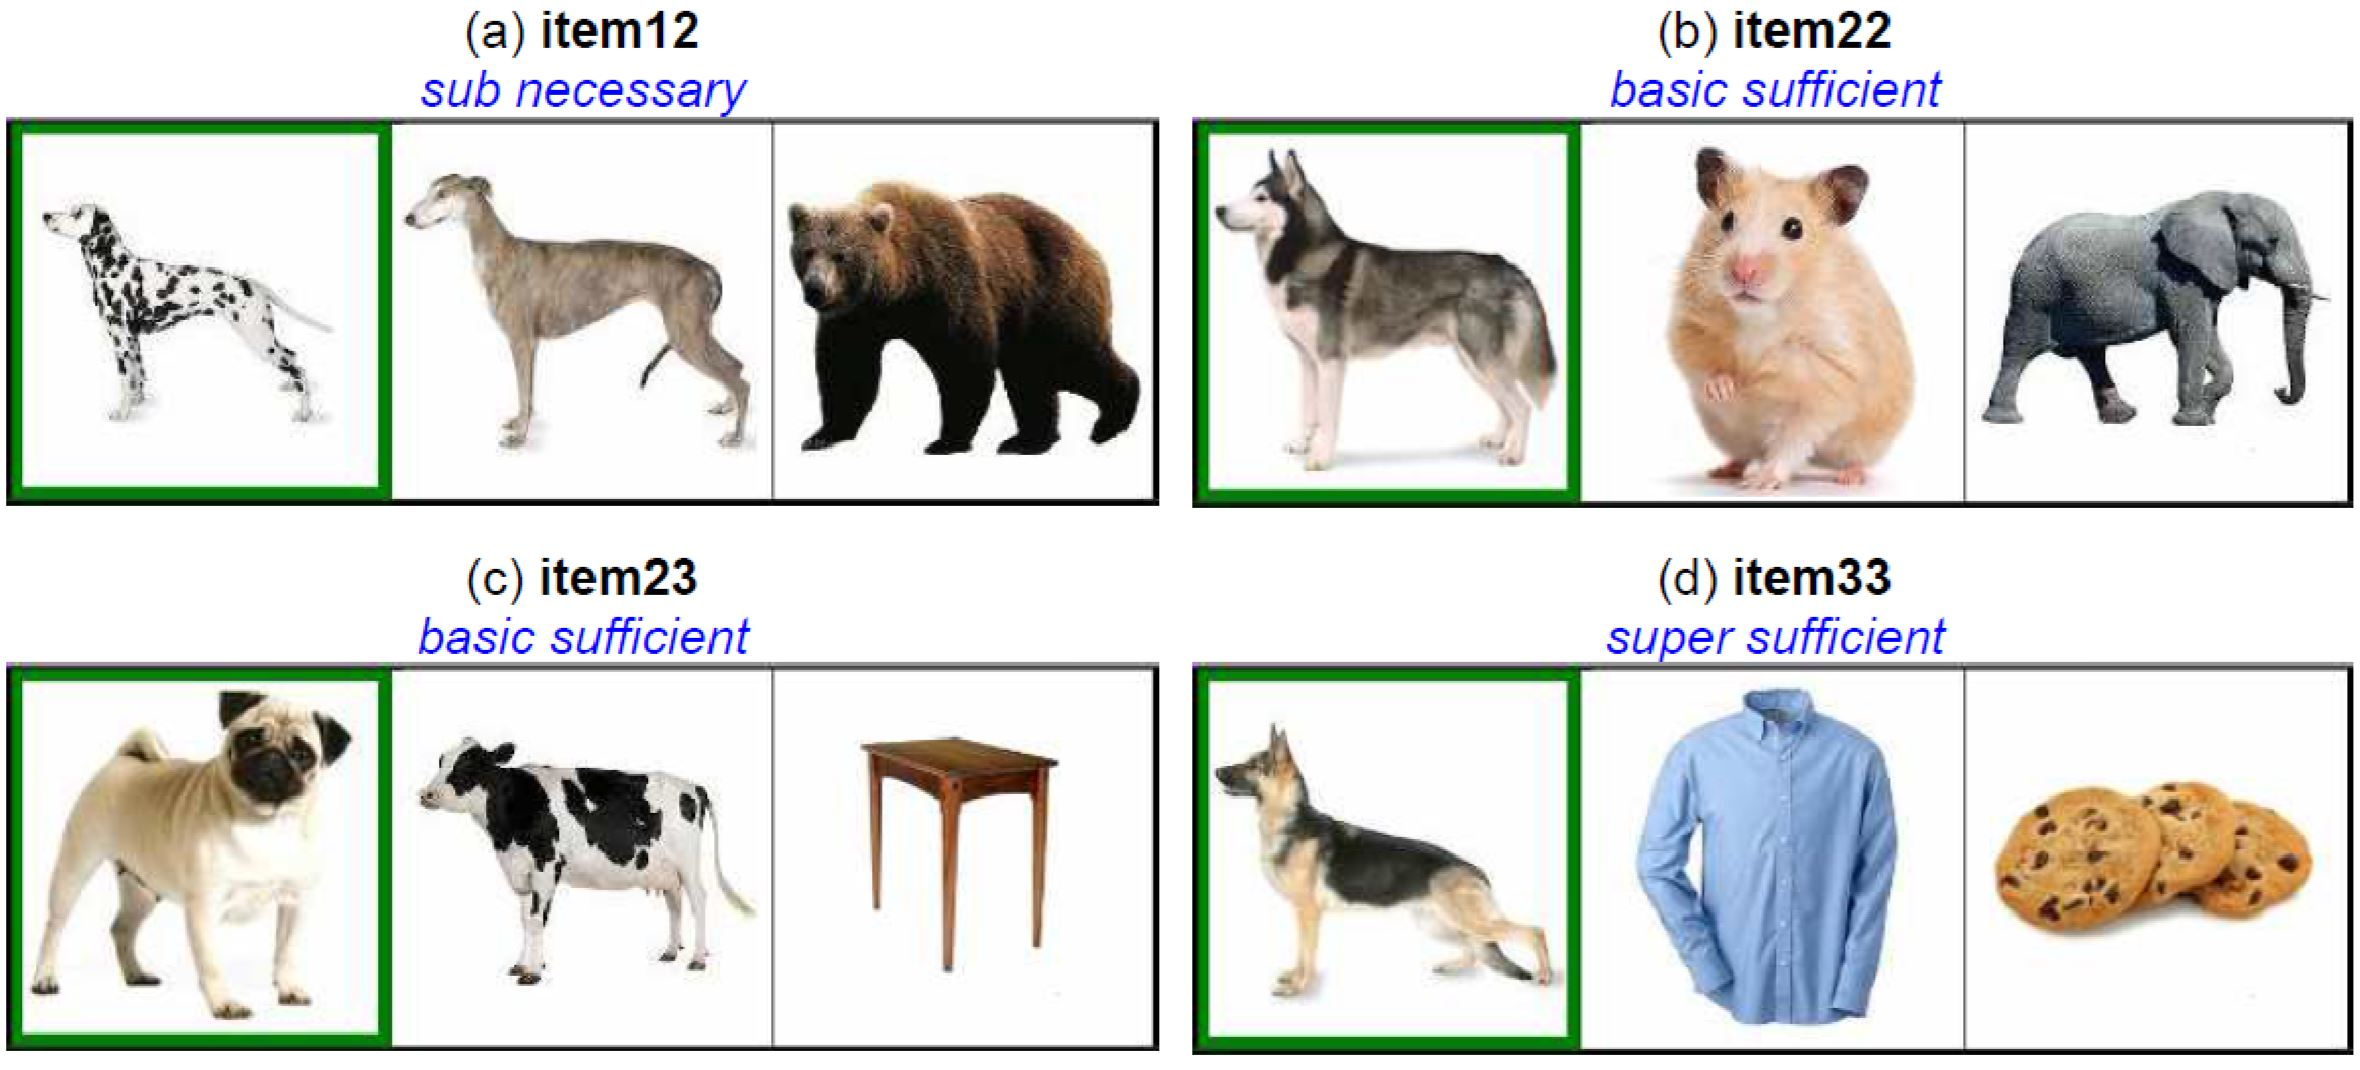
\includegraphics[width=4.2cm]{fig/graffig.jpg}
		\end{minipage}
		\begin{minipage}{.2\textwidth}
			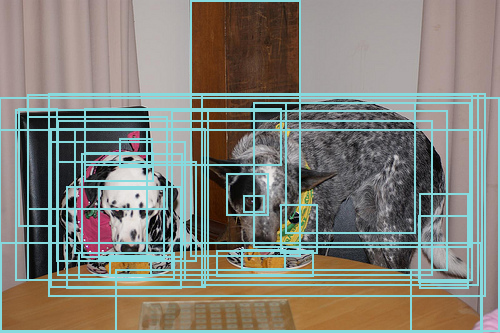
\includegraphics[height=2cm,width=2.5cm]{fig/visual_genome_dogs.png}
		\end{minipage}
	\begin{minipage}{.2\textwidth}
		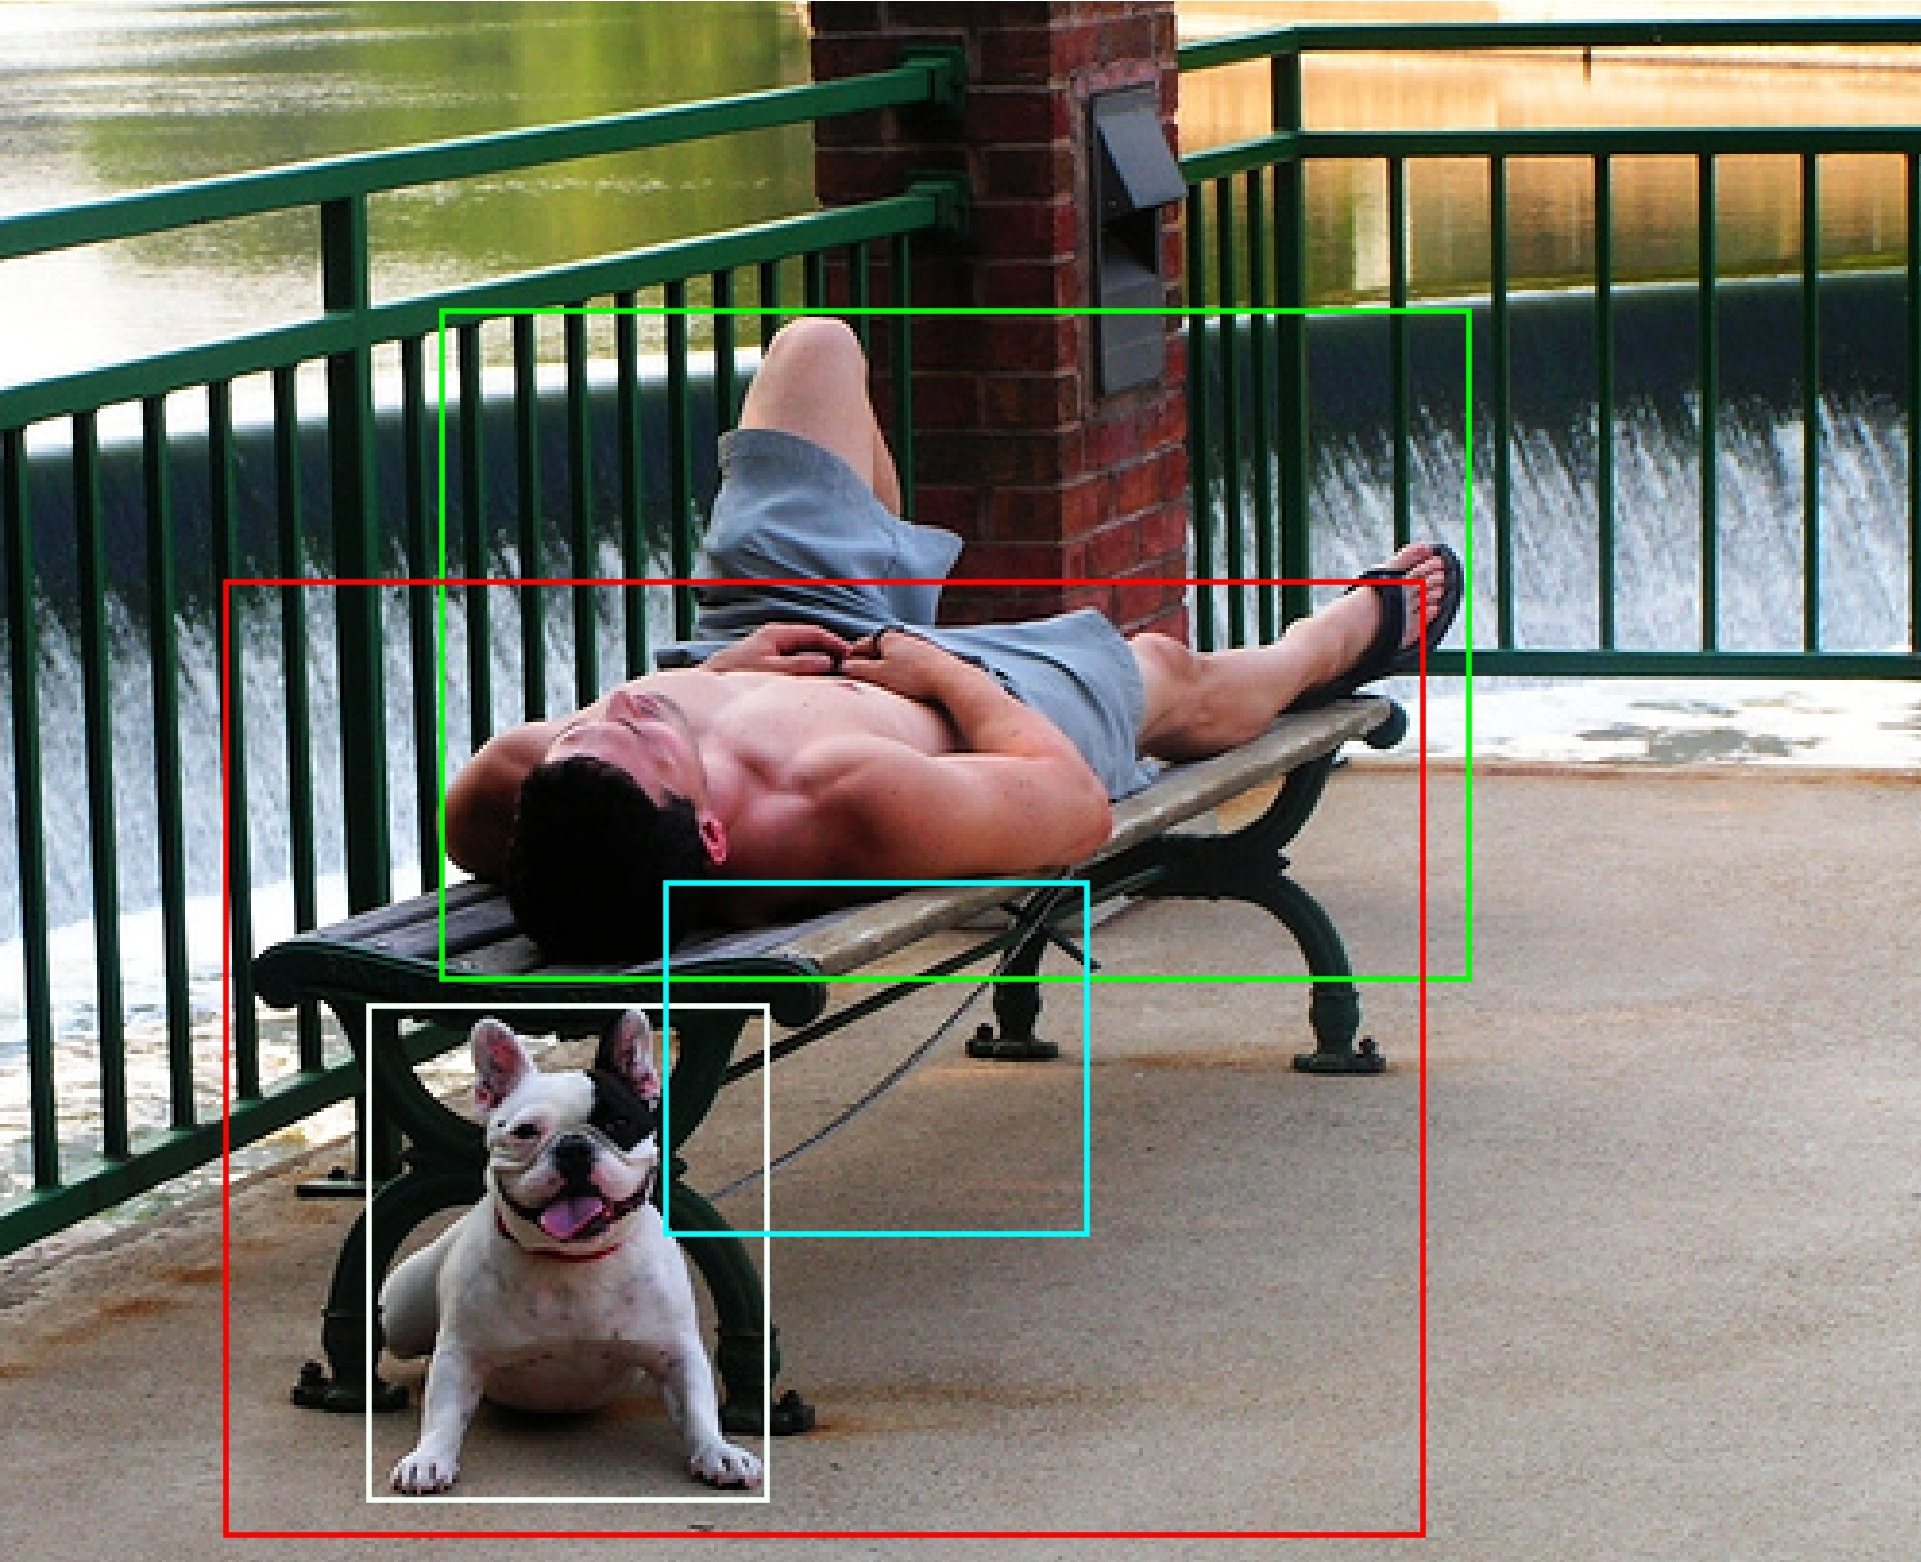
\includegraphics[height=2cm,width=2.5cm]{fig/flickr_1003163366_dog_boxes_crop.jpg}
	\end{minipage}
	\begin{minipage}{.2\textwidth}
		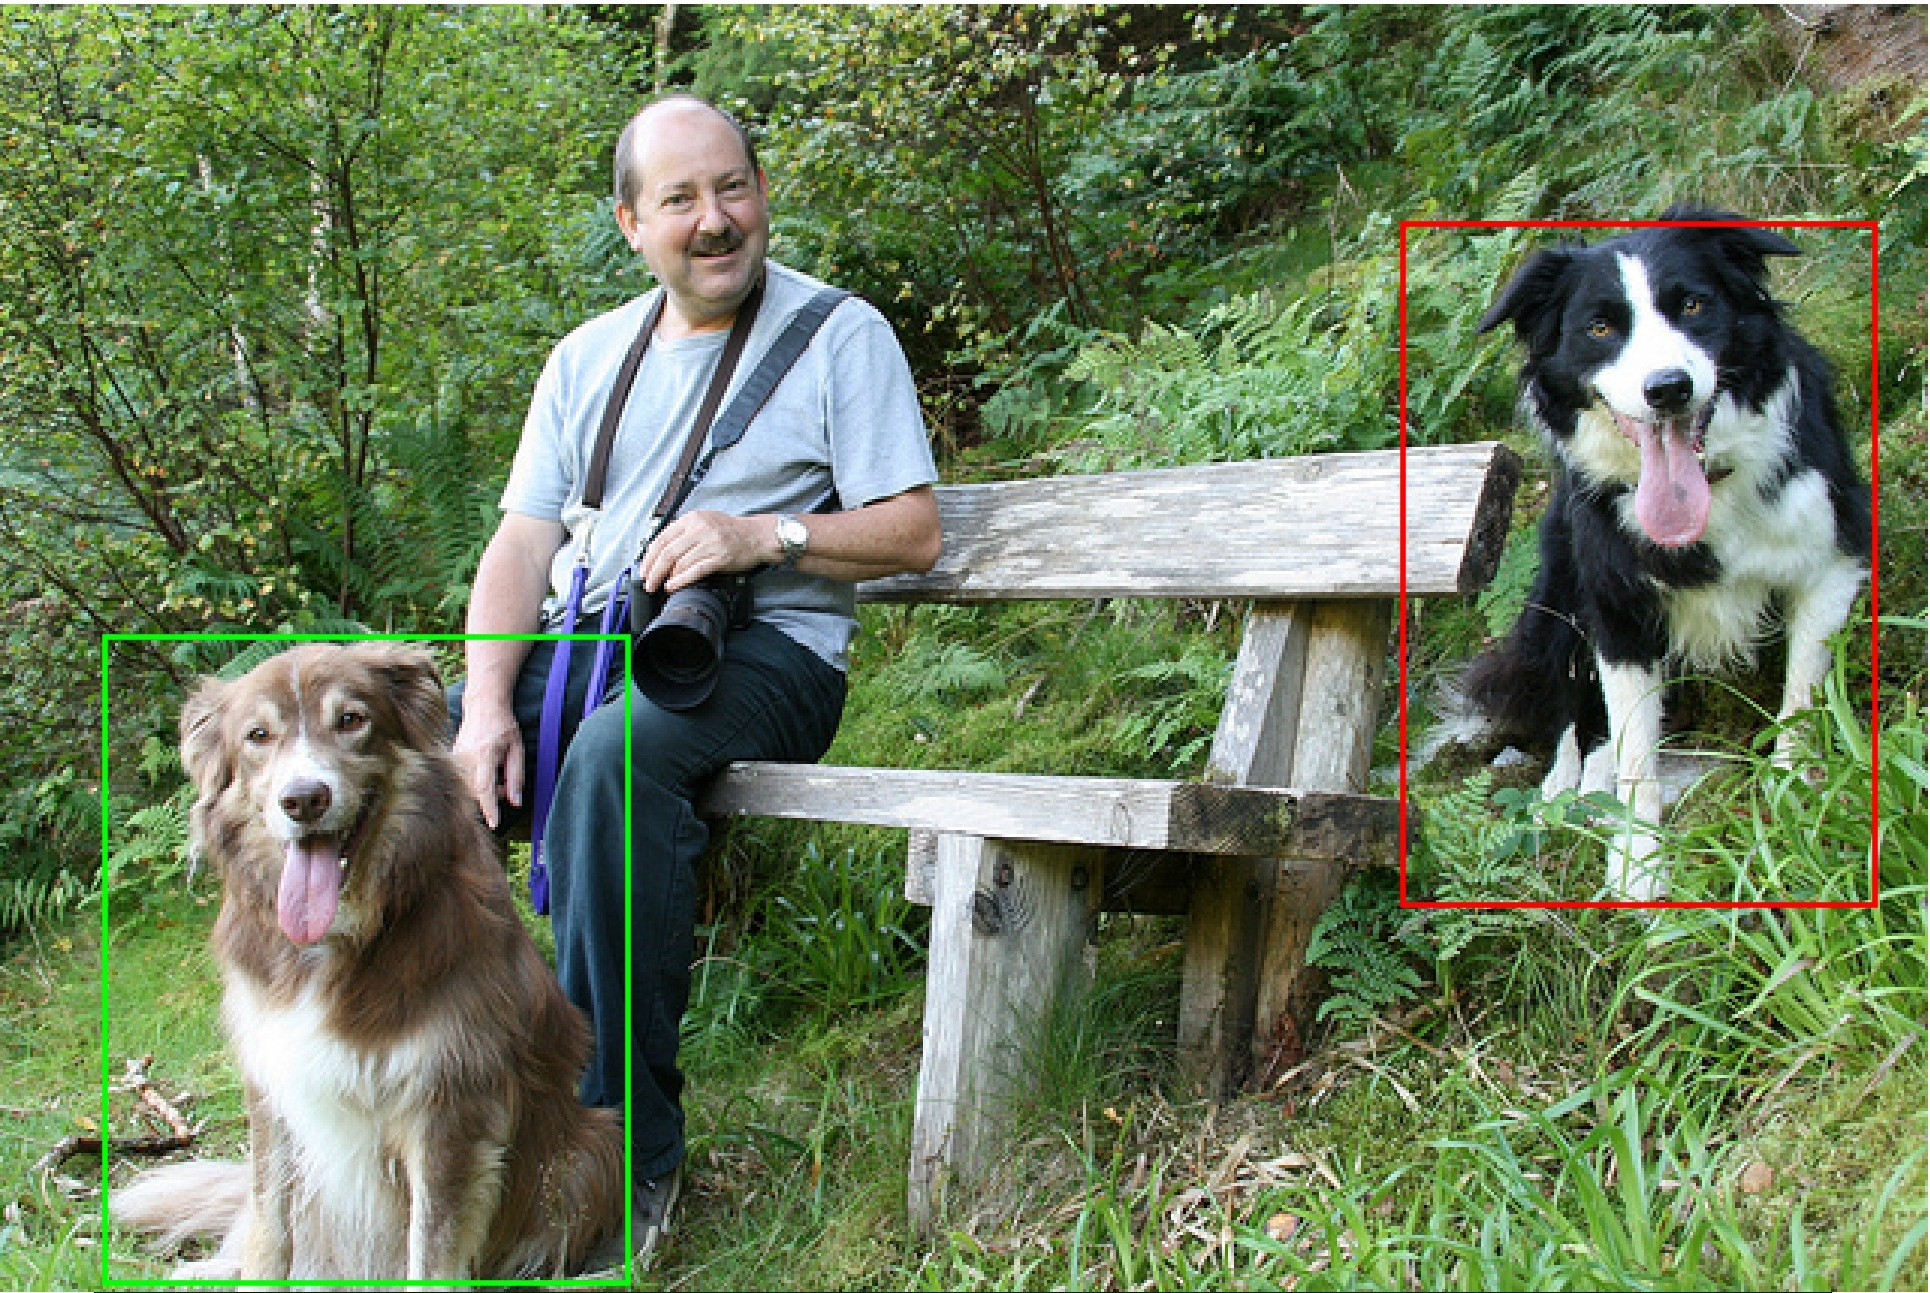
\includegraphics[height=2cm,width=2.5cm]{fig/refcoco_2400_dog_boxes_crop.jpg}
	\end{minipage}\vspace{-0cm}\\
\begin{minipage}{.35\textwidth}
	\tiny scene from  \cite{graf2016animal}
\end{minipage}
\begin{minipage}{.2\textwidth}
	\tiny
	{\textsl{dalmatian, dog, heeler}}
\end{minipage}
\begin{minipage}{.2\textwidth}
	\textsl{\tiny dog}
\end{minipage}
\begin{minipage}{.2\textwidth}
	\tiny \textsl{dog}
\end{minipage}
	\end{center}
		\vspace{-0.8cm}

	\caption{Experimental and real-world visual scenes showing dogs from Visual Genome, RefCoco, and Flickr)}
	\label{fig:graf_genome}
		\vspace{-0.5cm}

\end{figure}

In this Section we discuss the requirements for  being able to study the context dependence of object names in real-world images, inspired by \cite{graf2016animal}'s study.
 Figure \ref{fig:graf_genome} shows  \cite{graf2016animal}'s carefully controlled experimental conditions with isolated objects arranged in a collage, and real-world scenes where multiple objects occur in a natural context from \vgenome\cite{krishna2016visualgenome}, \refcoco\cite{Kazemzadeh2014}, and \flickr\cite{plummer2015flickr30kentities} (cf. Section~\ref{sec:resources}).
Thus, in contrast to \cite{graf2016animal} we do not aim for assembling controlled and, to some extent, artificial scenes, meaning that we need to be able to quantify contextual factors for naming in a real-world image corpus. 
Given a real-world scene with multiple objects and a target object that has to be named, we need access to:

\begin{itemize}   
		\item[(1)] the \textbf{specific category} of the object that the speaker referred to 
		\item[(2)] \textbf{exhaustive annotations} for all the other objects in the scene (i.e. distractors)
		\item[(3)] the \textbf{natural name} chosen by a speaker for referring to an object

\end{itemize}

%For instance, if we want to find out whether a specific object like \cat{convertible} is more often referred to with a basic-level category (e.g.,~\refexp{car}) or a more specific one (e.g.,~\refexp{convertible, limousine}), all three requirements need to be fulfilled: we need to know whether the object is a \cat{convertible} or a \cat{limousine}, and likewise for its distractors, and we need to know whether a speaker called the object \refexp{convertible, car, etc}.

For instance, if we want to find out whether a specific object like the left dog in  Fig.~\ref{fig:graf_genome}, second-left image, is more often referred to with a basic-level category (e.g.,~\refexp{dog}) or a more specific one (e.g.,~\refexp{dalmatian}), all three requirements need to be fulfilled: we need to know whether the object is a \cat{dalmatian} or, e.g.,~an \cat{irish setter}, and likewise for its distractors, and we need to know whether a speaker called the object \refexp{dalmatian, dog, etc}.


%\cs{Should the following be here or at the beginning of Sect. 4?}
%\cs{We could also call below requirements "Desiderata"}
%In practical terms, the prerequisite for Requirements~(2) and~(3) is, given an image, the information on \textbf{R1: the most specific category} of \textbf{each object} which is depicted in the image. 
%A taxonomy, such as WordNet \cite{fellbaum1998wordnet}, could then be queried with these categories to retrieve their individual lexical candidates arranged by their taxonomic relations. \\
%Furthermore, the information on the \textbf{R2: entry-level category} of an object could be used as a pivot to taxonomically group its lexical candidates.  
%Under the assumption that the entry-level, as the preferred level of specificity, is produced most often for an individual concept, may be inferrable from the data itself through maximum likelihood estimation. 
%For example, based on frequency estimates, the entry-level for the object on the left is \refexp{dalmatian} (Figure~\ref{fig:ex_visualgenome}), whereas the object on the right is named mostly \refexp{dog}, but \refexp{heeler} only once. 
%
%With respect to linguistic data-driven experiments, the range of linguistic phenomena under study (see, e.g.,~Section~\ref{sec:object_naming} for phenomena in object naming) need to be observable in the data in order to study the interaction of their underlying factors. 
%Hence, a further practical requirement is that the data, first, captures ideally all possible combinations of the factor values across all factors\footnote{For example, data that contains only images where target and distractor objects do not share any lexical candidates would not be appropriate}, and second, that it has been naturally produced in that speakers were not constraint in their choice of a name by external factors. 
%We summarize this requirement by the term \textbf{R3: unconstraint}. 
%Note that this requirement XXX \cs{@Sina ref to bias and paper you mentioned?}.
%


\section{Resources: What Do We Have?}
\label{sec:resources}

In the following, we will discuss datasets that provide descriptions or referring expressions for objects in real-world images and could, in principle,  be suitable for studying object naming. We focus on collections  that have been used for object recognition, referring expression generation, and phrase localization in previous work, but do not discuss other collections for e.g. image captioning which typically do not link mentions of objects to corresponding image regions.

\subsection{ImageNet}

ImageNet \cite{imagenet_cvpr09} is one of the biggest publicly available image databases and many state-of-the-art object recognizers are trained on a subsample of its categories (e.g.,~the ILSVRC image classification challenge comprises 1k synsets \cite{ILSVRC15}). 
ImageNet follows a consistent taxonomy as its hierarchical organization is based on WordNet \cite{fellbaum1998wordnet}, such that many synsets from WordNet can be queried for visual instances.
Vice versa, given a leaf node in the ImageNet hierarchy, all its specific and more general names can be retrieved by following the links between synsets in WordNet (as is actually done by \cite{Ordonez:2016}).
Many state-of-the-art object recognizers are trained on a subsample of ImageNet.
However, the database is not directly usable for our purposes as each image only depicts a single object (i.e. an instance of the synset) and no (or very few) distractor objects. 

\begin{table}
\centering
\setlength{\tabcolsep}{2pt}
\begin{tiny}
\begin{tabular}{rrl|rrl}
\toprule
 spec. &  rel.freq. &                          top 5 names & spec. &  rel.freq. &                          top 5 names \\
\midrule
           2 &   $<$ 0.01 &       \tiny                  thing,things & 10 &   0.05 &   elephant,couch,truck,vase,suitcase \\
           3 &   $<$ 0.01 &    object,group,set,substance,objects & 11 &   $<$ 0.01 &    motorcycle,clock,mom,dad,scissors \\
           4 &   0.14 &           man,person,piece,head,part & 12 &   $<$ 0.01 &  oven,airplane,suv,taxi,refrigerator  \\
           5 &   0.10 &       player,glass,baby,front,corner & 13 &   $<$ 0.01 &    laptop,fridge,canoe,orioles,pigeon \\
           6 &   0.21 &              woman,girl,kid,boy,bowl & 14 &   $<$ 0.01 &   panda,freezer,penguin,rooster,rhino \\
           7 &   0.25 &            guy,right,chair,lady,bear & 15 &   0.03 &    zebra,giraffe,zebras,giraffes,deer \\
           8 &   0.11 &           horse,bus,cow,pizza,batter & 16 &  $ <$ 0.01 &       bison,mooses,orang,elks,sambar \\
           9 &   0.09 &         shirt,car,bike,donut,catcher & 17 &   $<$ 0.01 &           ox,cattle,gnu,mustang,orca \\          
\bottomrule
\end{tabular}\caption{Levels of specificity for naming choices in RefCOCO: for each level (distance between name and WordNet root), relative frequency and 5 most frequent names are shown}
\label{tab:specnames}
\end{tiny}
\vspace{-1cm}
\label{tab:specnames}
\end{table}
\vspace{-0.6cm}


%Multiple datasets for vision \& language tasks have been built on top of COCO, such as the referring expressions datasets \refcoco and \refcocop which we will discuss below, and \textsl{COCO Captions} \cite{chen2015cococaptions}.  

\subsection{\refcoco and \refcocop \cite{Yu2016}}
Both datasets use the \referit\cite{Kazemzadeh2014} game for collecting referring expressions (RE) for natural objects in real-world images, and are built on top of the MS COCO \cite{mscoco}, 
%The latter provides five captions for each of  $300k$~images, spanning $80$~of the COCO categories.  
%However, the COCO region-level (object) annotations are not linked to the captions.
a dataset of images of natural scenes of $91$~common object categories (e.g.,~\cat{dog, pizza, chair}). 
The REs were collected via crowdsourcing in a two-player reference game designed to obtain REs uniquely referring to the target object. 
Specifically, a director and a matcher are presented with an image, and the director produces a RE for an outlined target object in the image. 
The matcher must click on the object he thinks the RE refers to. % (For more details on the datasets see \cite{Yu2016}). 
REs in \refcoco/+ were collected under the constraints that (i) all images contain at least two objects of the same category (80 COCO categories), which prompts the players to avoid the mere object category as RE, and (ii) in \refcocop the players must not use location words, urging them to refer to the appearance of objects. 
%Another critical property of the data is that, (iii), not all objects in an image were annotated with REs, may it due to the frequency constraint~(i), or due to the object not being part of the 80 COCO categories. 

\begin{itemize}
     		\item[(1)] \textbf{Specific categories}: not available, the $80$~COCO categories tend to be entry-level categories and are not linked to the ImageNet taxonomy (e.g.,~\cat{bird, person, car, bus})
		\item[(2)] \textbf{Exhaustive annotations}: not available, as not all objects were annotated with REs and corresponding categories
		   \item[(3)] \textbf{Natural names}: available, though it is unclear how the additional constraints in RefCoco+ impact on the naturalness of object naming
\end{itemize}

\paragraph{Analysis} We parse REs in \refcoco with the Stanford Dependency Parser and extract the nominal heads. We map these names to their most frequent sense/synset in WordNet.
We hypothesize that the distance of a name's synset to the root node (\cat{entity}) relates to its specificity.
We estimate this distance as the minimal path length of all synsets of a word  to the root node.
Table \ref{tab:specnames} shows the estimated levels of specificity for object names in the \refcoco data set.
We observe distances to the root between 2 and 17, meaning that there is a much more fine-grained distinction of levels than the three-way classification adopted in \cite{graf2016animal}.
Unfortunately, the levels of specificity predicted by WordNet do not seem to reflect linguistic intuitions, e.g.\ \refexp{elephant} is predicted to be more specific than \refexp{panda}.
At the same time, this overview clearly suggests that object names in \refcoco do not only comprise entry-level categories, but also very general (\refexp{thing}) and very specific names (\refexp{ox}).



\subsection{Flickr30k Entities}
The \flickr dataset \cite{plummer2015flickr30kentities}\footnote{Available at  \url{web.engr.illinois.edu/~bplumme2/Flickr30kEntities}}  augments Flickr30k, a dataset of 30k~images and five sentence-level captions for each of the images, with region-level annotations. 
Specifically, mentions of the same entities across the five captions of an image are linked to the bounding boxes of the objects they refer to. 
The dataset was designed to advance image description generation and phrase localization in particular (e.g.,~\cite{rohrbach2016grounding,plummer2017phrase,yeh2018unsupervised}). 

By design, \flickr can be used to study the way people refer to individual entities in an image depending on the situation the speakers describe and,  
in contrast to \refcoco/+, the production of entity mentions did not underlie any constraints. 
On the other hand, it is less suited for referring expression generation since mentions in isolation of their linguistic context may not uniquely identify the referred object. 

\begin{itemize}
     		\item[(1)] \textbf{Specific categories}: are not available, object categories tend to be even less specific than those of COCO (e.g.,~\cat{people, animals, bodyparts, clothing}), or are abstract (\cat{other, scene})
		\item[(2)] \textbf{Exhaustive annotations}: are not available
		   \item[(3)] \textbf{Natural names}: are available, though object names might not be fully discriminative (as in REs; e.g.,~both animals in the right-most image in Fig.~\ref{fig:graf_genome} are named \refexp{dog})

\end{itemize}

%\section{Carina}
%input{resources}

\subsection{Visual Genome}

\vgenome \cite{krishna2016visualgenome} aims to provide a full set of descriptions of the scenes which images depict in order to spur complete scene understanding. 
It contains a dense region-based labeling of $108k$~images with textual expression of the attributes and references of objects, their relationships as well as question answer pairs, all linked to WordNet synsets \cite[see below]{fellbaum1998wordnet}. 


\begin{itemize}
     		\item[(1)] \textbf{Specific categories}: are not available, as object categories and names are not consistently annotated (and even conflated)
				\item[(2)] \textbf{Exhaustive annotations}: are available, which is a huge advantage of this data sets
		   \item[(3)] \textbf{Natural names}: are available, though object names might not be fully discriminative (as in referring expressions)

\end{itemize}

\section{Possible Solutions}

As discussed in Section \ref{sec:resources}, none of the corpora that contain natural naming data for objects in context provide consistent and dense annotations of object categories at a sufficient level of specificity. We now discuss tentative solutions.

\subsection{Object detectors}
In order to obtain a sufficiently specific level for all objects in an image, an alternative would be to apply object detectors or image classifiers trained to predict the most specific category of the full inventory of objects which the dataset covers. 
However, pre-trained models only exist for a subset of the datasets' objects  (For example, we could find $6,139$~synsets for the unique object names of Flick30k, of which $238$~synsets (ss) are in the synset set of the ILSVRC image classification challenge ($1$K in total), and $338$ and $95$~ss are super-level and sub-level categories of ILSVRC, respectively.)
For the training of a model using, e.g., ImageNet \cite{imagenet_cvpr09}, on the other hand, the  set of most-specific categories covered by the data needs to be provided or collected from humans. 

%\subsection{Post-annotating COCO Captions}
%Regarding \refcoco/+, additional REs could be collected from the COCO Captions dataset. %, which provides 5 natural language descriptions for each image in MS COCO. 
%Since annotators could naturally refer to depicted objects in their descriptions (i.e.,~choose the entry-level as the most preferred reference whenever possible), we may infer the entry-level of the objects from them through maximum likelihood estimation. 
%%
%In contrast to \flickr, though, the data does not contain region-phrase associations,  % (i.e.,~object mentions are not linked to the corresponding image regions). 
%such that natural language phrases first needed to be aligned with the image regions they refer to. 
%This task of \textit{language grounding}, which has been an active research topic in vision \& language (e.g.,~\cite{kong2014what,karpathy2015deep,rohrbach2016grounding}), is beyond the focus of our object naming study. 
%% We could also examine the bias shift of speakers (e.g.,~sparrow vs. bird may depend on the person)
%
%

\subsection{Collect naming data with controlled level of specificity}

Given that the quality of exhaustive automatic object detection for arbitrary objects in our naming data is hard to estimate, further human annotation on some of the existing data sets seems to be required.
As annotation of arbitrary objects according to the ImageNet hierarchy is probably challenging for naive subjects, we plan to collect controlled, specific object names from humans as an approximate of specific categories.
Thus, by prompting annotators to label an object with the most specific name they can think of, we hope to be able to systematically gather object names at the sub-level.


%\label{sec:future_proposal}
%\textbf{TODO@Sina (?)}\\
%
 vision people have focussed on learning very specific categories, and have not cared about learning actual concepts/names, 
 
 language \& vision people have focussed on learning what speakers say in certain data sets, 
 we know that speakers will use object names at a medium level of specificity most of the time, 
 so it is difficult to learn the meaning of specific concepts from existing resources and to implement a model that can decide which level in the taxonomy is appropriate in context --- 
 we need a more systematic approach for collecting object naming data, 
 controlling the level of specificity (e.g. prompting speakers to come up with the most specific word they can think of)... this data might also give us insight into what basic-level and sub-level concepts are ..

%yes, will try ...

\section{Conclusion}

In this paper we have discussed some existing resources in vision \& language from the perspective of linguistically motivated studies on object naming.  
The comparison between different data sets and available annotations for them reveals that consistent procedures for annotating object categories and eliciting object names are lacking to an extent that testing of  basic linguistic hypotheses (related to the use of concepts) turns out to be difficult.



\clearpage
\bibliographystyle{splncs}
\begin{footnotesize}
\bibliography{naming}
\end{footnotesize}

\end{document}
